\documentclass[10pt,a4paper]{article}
\usepackage[utf8]{inputenc}
\usepackage{amsmath}
\usepackage{amsfonts}
\usepackage{amssymb}
\usepackage{makeidx}
\usepackage{graphicx}
\title{Conductor Borracho}
\date{Programación orientada a objetos }
\begin{document}
\maketitle

Implementar en el lenguaje de programación c++. En el juego hay dos protagonistas un conductor borracho y un policía, el objetivo del juego es que el policía atrape al conductor borracho. El juego se desarrollada con las siguientes características.

\begin{itemize}
	\item El tablero consta de una matriz de $11*11$ y este tiene unas barreras como se muestra a continuación
	\begin{center}
		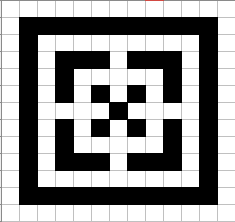
\includegraphics{board.png}
	\end{center}
	
	\item Cada jugador ocupa exactamente una casilla
	
	\item Cada jugada se hace oprimiendo la flecha hacia abajo
	\item Inicialmente el borracho aparece en el tablero, y después aparece el policía.
	
	\item Los turnos se van alternando uno para el borracho y uno para el policía
	
	\item Moviento jugadores:
	\begin{itemize}
		\item El movimiento normal del conductor borracho es el siguiente: tiene que escoger si moverse una o dos posiciones y escoger una dirección
		
		\item El movimiento normal del policía es el siguiente: se mueve una posición y escoge una dirección
	\end{itemize}
	En el caso de que no sea posible que el jugador se mueva en la dirección escogida se tiene que evaluar otra dirección teniendo en cuenta este orden: derecha, abajo, izquierda y arriba.
	\begin{flushleft}
		\textbf{Ejemplo:}
	\end{flushleft}
	\begin{itemize}
		\item Si el jugador escogió la derecha y no es posible entonces tiene que moverse hacia abajo.
		\item Si el jugador escogió arriba y no es posible entonces tiene que moverse hacia la derecha.
	\end{itemize}
	Esto pasos tienen que repetiste hasta que el jugador encuentre una dirección valida para moverse.
	\begin{flushleft}
		\textbf{Movimiento especial borracho}
	\end{flushleft}
	Si se da una situación como la que se muestra en el tablero, en la cual el conductor borracho escogió moverse hacia arriba con dos casillas, entonces se puede mover en diagonal, esto aplica para todo en todo el tablero y en todas la direcciónes cuando se da esta situacion.
	\begin{center}
		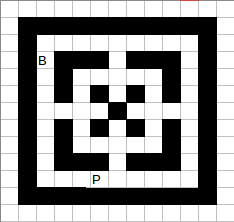
\includegraphics{boardMovedSpecial.png}
	\end{center}	
	\item Cuando el policía puede ver al borracho entonces en ese caso se mueve dos posiciones hacia el conductor borracho.
	\item En el caso en el que sea el turno sea del conductor borracho y el policía este a una casilla entonces el conductor borracho se mueve normalmente y deja una botella en donde estaba y  en el siguiente turno el policía tiene que coger la botella y pierde el turno de moverse.
	\item En el caso de que sea el turno del policía y el conductor borracho este a una o dos posiciones entonces en ese caso el juego termina.
	\item Es necesario mostrar las evaluaciones de la direcciones, las casilla para cada jugador, movimientos especiales, turno del jugador y cuando se termina el juego.
	
\end{itemize}

\end{document}